\documentclass[tikz,border=3.14mm]{standalone}
\usepackage{amsmath}
\usetikzlibrary{matrix,decorations.pathreplacing}
\usepackage{graphicx}
\begin{document}

	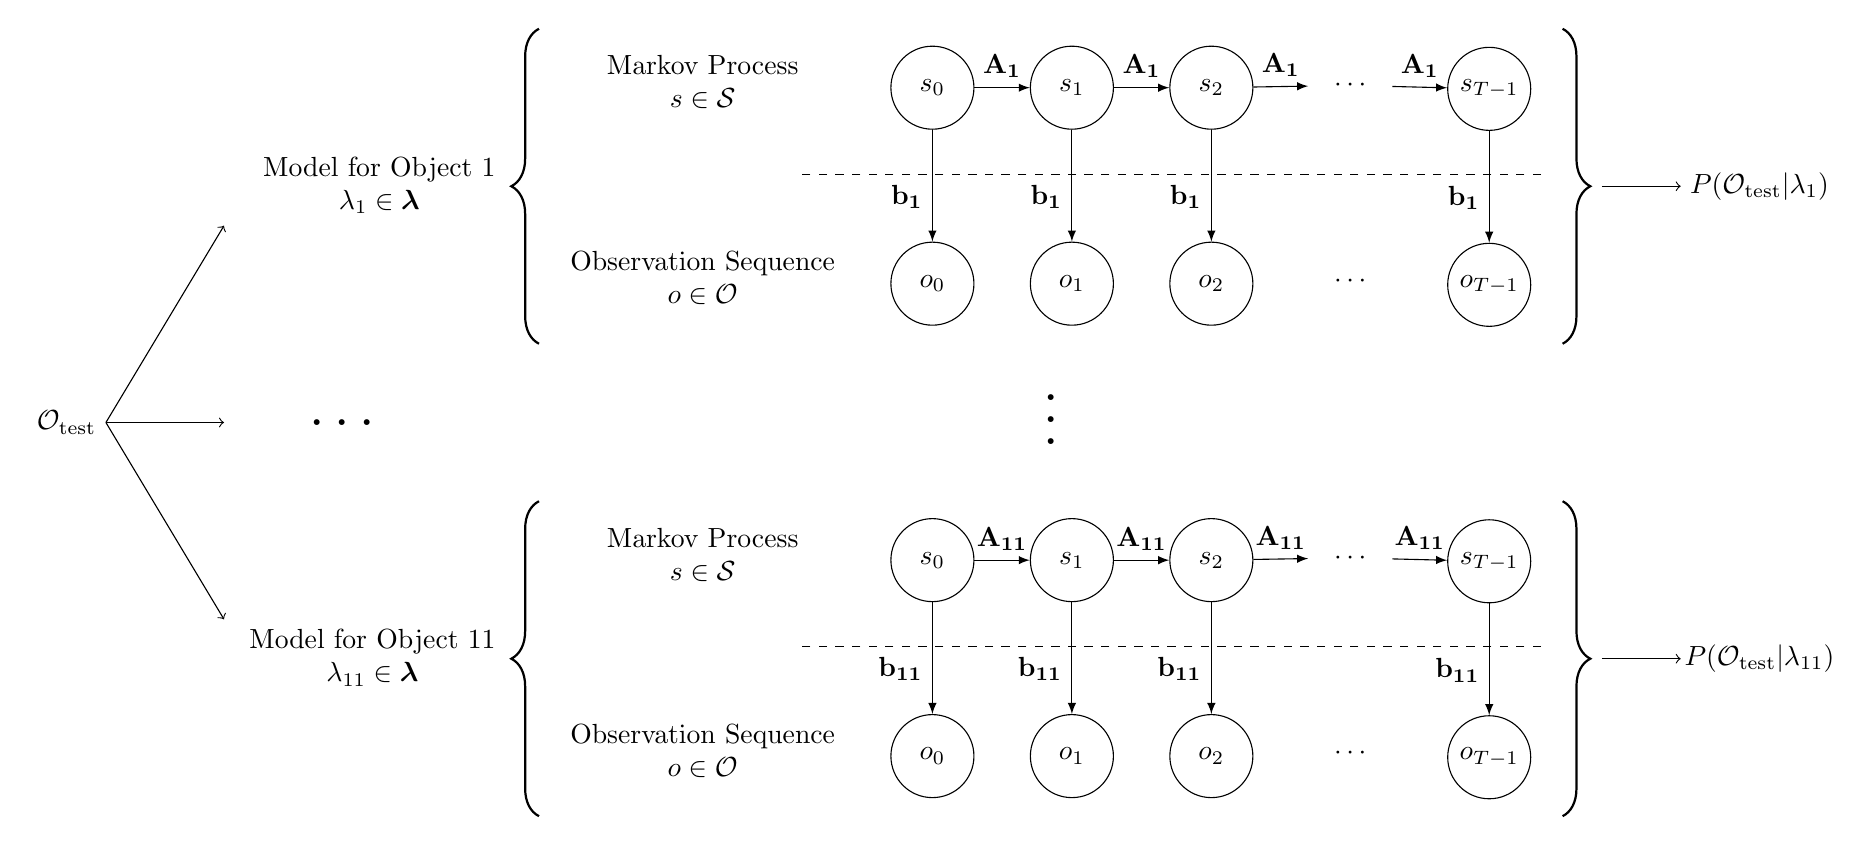
\begin{tikzpicture}
		\matrix (m1) at (0,0) [matrix of math nodes,column sep=2em,row sep=4em,cells= {nodes= {circle,draw,minimum width=3em,inner sep=0pt}}, column 1/.style= {nodes= {rectangle,draw=none}}, column 5/.style= {nodes= {rectangle,draw=none}}] (m) {
			\text{$\begin{matrix}\text{Markov Process}\\\text{$s \in \mathcal{S}$}\end{matrix}$} & s_0 & s_1 & s_2 & \cdots & s_{T-1}\\
			\text{$\begin{matrix}\text{Observation Sequence}\\\text{$o \in \mathcal{O}$}\end{matrix}$} & o_0 & o_1 & o_2 & \cdots & o_{T-1}\\
		};
		\foreach \X in {2,3,4,5} {
			\draw [-latex] (m-1-\X) -- (m-1-\the\numexpr\X+1) node [midway,above] {$\mathbf{A_1}$};
			\ifnum\X=5
			\draw [-latex] (m-1-6) -- (m-2-6) node [pos=0.6,left] {$\mathbf{b_1}$};
			\else
			\draw [-latex] (m-1-\X) -- (m-2-\X) node [pos=0.6,left] {$\mathbf{b_1}$};
			\fi
		}
		\draw [dashed] ([yshift=1ex]m.east) -- ([yshift=1ex]m.east-|m-1-1.east);
		
		% Add big square brackets
		\draw [thick, decorate, decoration={brace,amplitude=10pt, mirror}] 	(-6.5,2) -- (-6.5,-2) node[midway,left=12pt] {$\begin{matrix}\text{Model for Object 1}\\\text{$\lambda_1 \in \boldsymbol{\lambda}$}\end{matrix}$};
		\draw [thick, decorate, decoration={brace,amplitude=10pt}] 	(6.5, 2) -- (6.5, -2);
		
		\node at (0,-2.75) {\scalebox{2}{$\vdots$}};

		\matrix (m1) at (0,-6) [matrix of math nodes,column sep=2em,row sep=4em,cells= {nodes= {circle,draw,minimum width=3em,inner sep=0pt}}, column 1/.style= {nodes= {rectangle,draw=none}}, column 5/.style= {nodes= {rectangle,draw=none}}] (m) {
			\text{$\begin{matrix}\text{Markov Process}\\\text{$s \in \mathcal{S}$}\end{matrix}$} & s_0 & s_1 & s_2 & \cdots & s_{T-1}\\
			\text{$\begin{matrix}\text{Observation Sequence}\\\text{$o \in \mathcal{O}$}\end{matrix}$} & o_0 & o_1 & o_2 & \cdots & o_{T-1}\\
		};
		\foreach \X in {2,3,4,5} {
			\draw [-latex] (m-1-\X) -- (m-1-\the\numexpr\X+1) node [midway,above] {$\mathbf{A_{11}}$};
			\ifnum\X=5
			\draw [-latex] (m-1-6) -- (m-2-6) node [pos=0.6,left] {$\mathbf{b_{11}}$};
			\else
			\draw [-latex] (m-1-\X) -- (m-2-\X) node [pos=0.6,left] {$\mathbf{b_{11}}$};
			\fi
		}
		\draw [dashed] ([yshift=1ex]m.east) -- ([yshift=1ex]m.east-|m-1-1.east);
		
		% Add big square brackets
		\draw [thick, decorate, decoration={brace,amplitude=10pt, mirror}] 	(-6.5,-4) -- (-6.5,-8) node[midway,left=12pt] {$\begin{matrix}\text{Model for Object 11}\\\text{$\lambda_{11} \in \boldsymbol{\lambda}$}\end{matrix}$};
		\draw [thick, decorate, decoration={brace,amplitude=10pt}] 	(6.5,-4) -- (6.5,-8);
		
		%add arrows pointing to models
		\draw[->, out=150, in=30]        (-12,-3)   -- (-10.5,-0.5);
		\draw[->]        (-12,-3)   -- (-10.5,-5.5);
		\draw[->]        (-12,-3)   -- (-10.5,-3);
		\node (dots) at (-9,-3) {\scalebox{2}{$\hdots$}};
		\node (input) at (-12.5,-3) {$\mathcal{O}_{\text{test}}$};
		
		\draw[->]        (7,0)   -- (8,0);
		\draw[->]        (7,-6)   -- (8,-6);
		\node (input) at (9,0) {$P(\mathcal{O}_{\text{test}}|\lambda_{1})$};
		\node (input) at (9,-6) {$P(\mathcal{O}_{\text{test}}|\lambda_{11})$};
	\end{tikzpicture}
	
\end{document}
